\section{Строгие полы индекса: объёмный, инрадиусный и оболочечный экраны}
\label{sec:floors}

Насколько далеко можно спуститься по числу цветов на данном родителе? Три
экрана дают строгие нижние границы индекса, привязанные к конкретной
родительской решётке, без всякого перебора подрешёток.

\subsection{Объёмный экран Минковского}\label{ssec:mink}

Условие правильности раскраски $D(v)\ge\diam V_0$ для всех $v\in\Gamma
\setminus\{0\}$ равносильно геометрическому утверждению
\[
\Gamma\cap\operatorname{int}K=\{0\},\qquad K=2\bigl(V_0\oplus R\,B\bigr),
\]
где $R$ --- радиус покрытия, $B$ --- единичный шар. Тело $K$ центрально
симметрично и выпукло как сумма Минковского симметричного многогранника и шара,
поэтому применима теорема Минковского о выпуклом теле.

\begin{proposition}[объёмная нижняя граница индекса]\label{prop:mink}
Для любой подрешётки $\Gamma\subset\Lambda$, задающей правильную
раскраску,
\begin{equation}\label{eq:mink}
k=[\Lambda:\Gamma]\ \ge\ \frac{\vol\bigl(V_0\oplus R\,B\bigr)}{\det\Lambda}\,,
\end{equation}
и, по неравенству Брунна--Минковского, в замкнутой форме
$k\ge\bigl(1+R\,\omega_n^{1/n}/(\det\Lambda)^{1/n}\bigr)^n$, где $\omega_n$ ---
объём единичного шара.
\end{proposition}

\begin{proof}
Из $\Gamma\cap\operatorname{int}K=\{0\}$ по теореме Минковского
$\vol K\le2^n\det\Gamma$; при этом $\vol K=2^n\vol(V_0\oplus RB)$, откуда
$\det\Gamma\ge\vol(V_0\oplus RB)$, что и есть~\eqref{eq:mink}. Замкнутая форма
получается из $\vol(V_0\oplus RB)^{1/n}\ge(\det\Lambda)^{1/n}+R\,\omega_n^{1/n}$.
\end{proof}

Раньше минимальность индекса на фиксированном родителе устанавливалась
только исчерпывающим перебором (например, $1\,424\,115\,231$ подрешёток
индекса $140$ в $A_5^*$, \S\ref{sec:identity}). Ценность~\eqref{eq:mink} ---
диагностическая: отношение достигнутого индекса к правой части показывает,
насколько конструкция далека от объёмного препятствия:

\begin{center}\small
\begin{tabular}{c l r r r}
\toprule
$n$ & решётка & граница~\eqref{eq:mink} & известный $k$ & отношение\\
\midrule
2 & $A_2$    & $4{,}51$   & $7$     & $1{,}55$\\
3 & $A_3^*$  & $10{,}42$  & $15$    & $1{,}44$\\
4 & $D_4$    & $28{,}88$  & $49$    & $1{,}70$\\
5 & $A_5^*$  & $55{,}55$  & $140$   & $2{,}52$\\
6 & $E_6^*$  & $127{,}86$ & $343$   & $2{,}68$\\
7 & $E_7^*$  & $340{,}2$  & $1372$  & $4{,}03$\\
8 & $E_8$    & $663{,}9$  & $2401$  & $3{,}62$\\
9 & $A_9^*$  & $1639{,}7$ & $17253$ & $\mathbf{10{,}52}$\\
\bottomrule
\end{tabular}
\end{center}

\noindent Размерность~$9$ --- очевидный выброс: ей не хватало не оптимизации,
а \emph{конструкции}, и именно эту диагностику закрыли ламинирование
(\S\ref{sec:lam}) и продуктовое правило~\cite{Bounds}. Отметим сразу и
ограничение экрана: он оценивает потенциал, но не достижимость. Так, для
$A_7^*$ граница~\eqref{eq:mink} равна $300{,}7$ против $340{,}2$ у $E_7^*$,
однако наилучший найденный индекс на $A_7^*$ равен $2016$ --- заметно хуже, чем
$1323$ на деформированной $E_7^*$~\cite{Full}.

\subsection{Инрадиусный экран: плоский блок индекса 19 неулучшаем}
\label{ssec:planefloor}

Рядом с $E_8/2401$ плоский блок обязан иметь $d\ge\sqrt7$ (бюджет $1/7$,
оставленный блоком $E_8/2401$, требует ровно $1/d^2\le1/7$). Полный перебор
показывает, что впервые это достигается при $k=19$: перебираются все формы
Эрмита индекса~$k$ (их $\sigma(k)$) и все формы плоских решёток с точностью до
подобия (двупараметрическое семейство; максимизация численная). Индексы
$16,17,18$ дают $2{,}598$, $2{,}520$, $2{,}479$.

Нижняя часть диапазона закрывается доказательно, причём двумя дополняющими
экранами. Первый --- объёмный (\S\ref{ssec:mink}): $k\ge\vol(V_0\oplus
(\ell\diam/2)B)/\det\Lambda$, что на шестиугольной решётке даёт $15{,}574$.
Второй --- новый.

\begin{proposition}[инрадиусный экран]\label{prop:inrfloor}
Для допустимой при ширине $\ell$ пары $\Gamma\subset\Lambda\subset\R^n$
\[
k=[\Lambda:\Gamma]\ \ge\ \frac{(\ell\,\diam V_0+\lambda_1)^n}
{\gamma_n^{n/2}\,\det\Lambda}.
\]
\end{proposition}

\begin{proof}
Инрадиусная лемма~\ref{lem:inradius} даёт $D(v)\le|v|-\lambda_1$, поэтому
допустимость влечёт $\lambda_1(\Gamma)\ge\ell\diam V_0+\lambda_1$. Неравенство
Эрмита $\lambda_1(\Gamma)^n\le\gamma_n^{n/2}\det\Gamma$ и
$\det\Gamma=k\det\Lambda$ дают требуемое.
\end{proof}

Этот экран \emph{не следует} из объёмного и в плоскости при $\ell=\sqrt7$
сильнее: $16{,}443$ против $15{,}574$ на шестиугольной решётке. Оба верны для
каждой формы решётки, поэтому строгий пол есть минимум по формам от максимума
двух экранов; скан пространства модулей с последующей доводкой даёт $16{,}021$
(при $x=-0{,}5$, $y=1{,}0754$). Итог: \emph{индекс $k\le16$ невозможен
доказательно}, а $k=17,18$ исключены пока лишь численно.

\begin{figure}[htbp]\centering
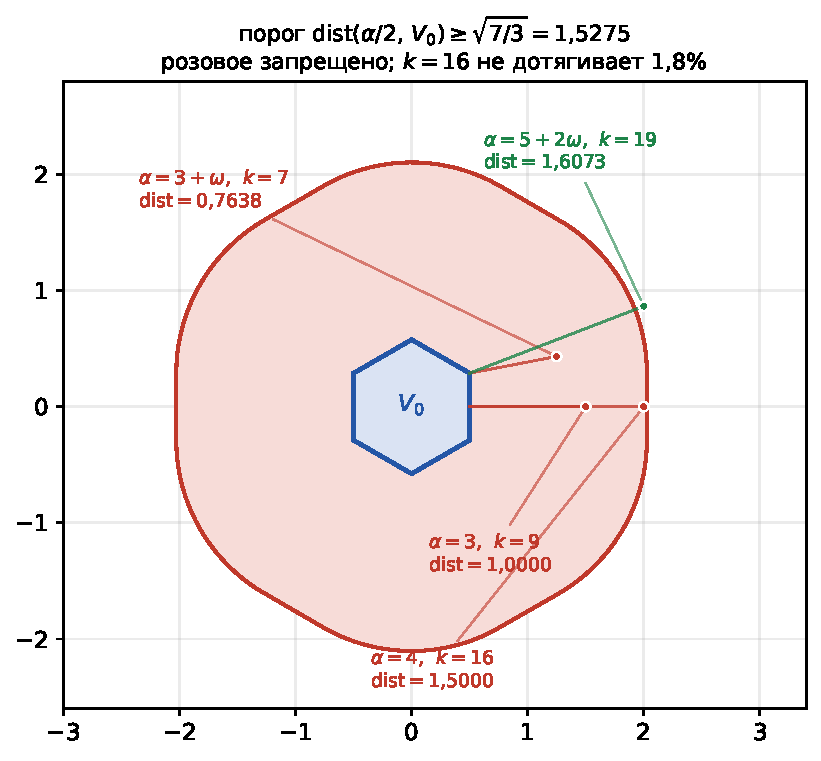
\includegraphics[width=0.72\textwidth]{fig_spacer.pdf}
\caption{Почему плоский проставок стоит ровно~19. Синий шестиугольник --- ячейка
$V_0$ решётки $A_2$; розовая область --- её окрестность радиуса
$\sqrt{7/3}=1{,}5275$, куда точка $\alpha/2$ попадать не должна. Отрезки ведут к
ближайшей точке ячейки. Индекс~16 ($\alpha=4$) не дотягивает $1{,}8\%$, и лишь
$\alpha=5+2\omega$ выходит наружу.}
\label{fig:spacer}
\end{figure}

\subsection{Оболочечный экран: когда пол совпадает с рекордом}
\label{ssec:shellfloor}

Инрадиусный экран останавливается на неравенстве
$\lambda_1(\Gamma)\ge\ell\diam V_0+\lambda_1$ и дальше пользуется только им.
Но норма вектора решётки пробегает не континуум, а \emph{оболочки}; если первая
оболочка над этим порогом запрещена целиком, то $\lambda_1(\Gamma)^2$
поднимается скачком до следующей, и пол растёт вместе с ней. На сильно
симметричных решётках выигрыш оказывается решающим: пол \emph{совпадает} с
рекордом, то есть рекорд на этом родителе неулучшаем.

\begin{proposition}[оболочечный экран]\label{prop:shellfloor}
Пусть $s^{\ast}>0$ таково, что каждый $v\in\Lambda\setminus\{0\}$ с
$|v|^2<s^{\ast}$ удовлетворяет $D(v)<\ell\diam V_0$. Тогда для допустимой при
ширине $\ell$ пары $\Gamma\subset\Lambda\subset\R^n$
\[
k=[\Lambda:\Gamma]\ \ge\ \frac{(s^{\ast})^{n/2}}{\gamma_n^{n/2}\det\Lambda}.
\]
\end{proposition}

\begin{proof}
Допустимость означает $D(v)\ge\ell\diam V_0$ для всех $v\in\Gamma\setminus\{0\}$,
поэтому по условию $|v|^2\ge s^{\ast}$, то есть
$\lambda_1(\Gamma)^2\ge s^{\ast}$. Дальше --- неравенство Эрмита
$\lambda_1(\Gamma)^n\le\gamma_n^{n/2}\det\Gamma$ и $\det\Gamma=k\det\Lambda$,
как в предложении~\ref{prop:inrfloor}.
\end{proof}

Работает предложение ровно настолько, насколько удаётся доказывать запрет
оболочек. Здесь достаточно однострочного свидетеля.

\begin{lemma}[радиальный свидетель]\label{lem:radial}
Пусть $\langle\Lambda,\Lambda\rangle\subseteq\frac1e\Z$, пусть $|v|^2=N$
и пусть рациональное $s\in(0,\tfrac12)$ таково, что для каждой оболочки
$|u|^2=M<4s^2N$ выполнено
\[
s\cdot\frac{\bigl\lfloor e\sqrt{NM}\bigr\rfloor}{e}\ \le\ \frac M2 .
\]
Тогда $sv\in V_0$ и, следовательно,
$D(v)\le2\bigl(\tfrac12-s\bigr)\sqrt N$.
\end{lemma}

\begin{proof}
Ячейка есть $V_0=\{x:\langle x,u\rangle\le|u|^2/2\ \forall u\in\Lambda\}$, так
что надо проверить $s\langle v,u\rangle\le|u|^2/2$. При $|u|^2=M\ge4s^2N$ это
даёт уже неравенство Коши--Буняковского: $s\langle v,u\rangle\le s\sqrt{NM}\le
M/2$, поскольку последнее равносильно $M\ge4s^2N$. Оболочек с $M<4s^2N$ конечно
много, и на них к Коши--Буняковскому добавляется целочисленность: $\langle
v,u\rangle$ кратно $1/e$ и не превосходит $\sqrt{NM}$, значит не превосходит
$\lfloor e\sqrt{NM}\rfloor/e$; это и есть условие леммы. Наконец
$D(v)=2\dist(v/2,V_0)\le2|v/2-sv|=2(\tfrac12-s)\sqrt N$.
\end{proof}

Ни перечисления векторов, ни численного счёта здесь нет: нужен только
\emph{спектр} норм решётки. Этого хватает, чтобы закрыть две размерности.

\begin{keybox}
\begin{theorem}[$2401$ неулучшаемо на $E_8$]\label{thm:e8opt}
Пусть $\Lambda=E_8$ (минимум~$2$, $R_{\mathrm{cov}}=1$,
$\det\Lambda=1$) и пара $\Gamma\subset\Lambda$ допустима при $\ell=1$. Тогда
$[\Lambda:\Gamma]\ge2401$, и равенство достигается на
$\Gamma=(3+\omega)E_8$.
\end{theorem}
\end{keybox}

\begin{proof}
Инрадиусная лемма~\ref{lem:inradius} даёт
$|v|\ge\diam V_0+\lambda_1=2+\sqrt2$, то есть $|v|^2\ge6+4\sqrt2=11{,}6568\ldots$
Решётка $E_8$ чётная, поэтому $|v|^2\in2\Z$ и ближайшая возможность ---
$|v|^2=12$.

Пусть $|v|^2=12$. Применим лемму~\ref{lem:radial} с $e=1$ и $s=\tfrac14$: тогда
$4s^2N=3$, так что отдельной проверки требует единственная оболочка $M=2$, а на
ней $\lfloor\sqrt{24}\rfloor=4$ (ибо $\sqrt{24}=4{,}898\ldots$) и
$\tfrac14\cdot4=1\le\tfrac22$. Значит $v/4\in V_0$ и
\[
D(v)\ \le\ 2\Bigl(\tfrac12-\tfrac14\Bigr)\sqrt{12}\ =\ \sqrt3\ <\ 2\ =\ \diam V_0 .
\]
Оболочка $12$ запрещена целиком, поэтому $s^{\ast}=14$. Предложение
\ref{prop:shellfloor} с $\gamma_8=2$ (Блихфельдт) даёт
$k\ge14^4/2^4=7^4=2401$.

Равенство: у $(3+\omega)E_8$ индекс $N(3+\omega)^4=7^4=2401$ и
$\lambda_1^2=7\cdot2=14$, а подобие $E_8$ обращает неравенство Эрмита в
равенство.
\end{proof}

\begin{keybox}
\begin{theorem}[$15$ неулучшаемо на ОЦК]\label{thm:a3opt}
Пусть $\Lambda=A_3^{*}$ (ОЦК; $\lambda_1^2=3/4$,
$R_{\mathrm{cov}}^2=5/16$, $\det\Lambda=1/2$) и пара $\Gamma\subset\Lambda$
допустима при $\ell=1$. Тогда $[\Lambda:\Gamma]\ge15$.
\end{theorem}
\end{keybox}

\begin{proof}
Инрадиусная лемма даёт $|v|^2\ge(2R_{\mathrm{cov}}+\lambda_1)^2=
2+\tfrac{\sqrt{15}}2=3{,}9364\ldots$ Нормы ОЦК суть целые числа и числа вида
(сумма трёх нечётных квадратов)$/4$, поэтому в окне
$[3{,}9364,\ (2\diam V_0)^2=5]$ лежат ровно три оболочки: $4$, $19/4$ и $5$.
Оболочка~$4$ запрещена леммой~\ref{lem:radial} с $e=4$, $s=\tfrac14$: тогда
$4s^2N=1$, отдельно проверяется лишь $M=3/4$, где
$\lfloor4\sqrt3\rfloor/4=6/4$ и $\tfrac14\cdot\tfrac64=\tfrac38=\tfrac M2$;
отсюда $D(v)\le2\cdot\tfrac14\cdot2=1<\sqrt{5}/2=\diam V_0$. Значит
$s^{\ast}=19/4$, и предложение~\ref{prop:shellfloor} с
$\gamma_3^{3/2}=\sqrt2$ даёт $k^2\ge(19/4)^3/\tfrac12=6859/32$, то есть
$k\ge14{,}64\ldots$ и $k\ge15$.
\end{proof}

Для ОЦК граница $15$ известна: её даёт общая теорема Кулсона
$\chi_s\ge2^{n+1}-1$ \cite{Coulson}; новое здесь --- вывод из одного лишь
спектра норм. Для $E_8$ же граница $2401$ нова: теорема Кулсона даёт только
$2^9-1=511$. Тем самым оболочечный экран отвечает --- для отдельных решёток
--- на открытый вопрос~8 работы~\cite{ABPR} о нижних границах, зависящих
от дополнительных характеристик решётки.

Сводка по классическим родителям (столбец <<было>> --- инрадиусный экран
предложения~\ref{prop:inrfloor}, то есть тот же счёт при
$s^{\ast}=(\diam V_0+\lambda_1)^2$):

\begin{center}\small
\begin{tabular}{lccccrrc}
\toprule
$\Lambda$ & $n$ & $\lambda_1^2$ & оболочки в окне & $s^{\ast}$ &
было & стало & рекорд\\
\midrule
$A_3^{*}$ & $3$ & $3/4$ & $4,\ 19/4,\ 5$ & $19/4$ & $11$ & $\mathbf{15}$ & $15$\\
$E_6^{*}$ & $6$ & $4/3$ & $8,\ 28/3,\ 10$ & $28/3$ & $176$ & $\mathbf{305}$ & $343$\\
$E_8$ & $8$ & $2$ & $12,\ 14,\ 16$ & $14$ & $1154$ & $\mathbf{2401}$ & $2401$\\
$K_{12}$ & $12$ & $4$ & $28,\ 30,\ \ldots$ & $30$ & $111\,019$ & $\mathbf{177\,979}$ & $3^{12}$\\
$\Lambda_{24}$ & $24$ & $4$ & $24,\ 26,\ \ldots$ & $26$ & --- & $\mathbf{5\,688\,009\,064}$ & $7^{12}$\\
\bottomrule
\end{tabular}
\end{center}

\noindent
Строки $K_{12}$ и $\Lambda_{24}$ получены вообще без перечисления: обе решётки
чётные с минимумом~$4$, то есть спектр норм равен $\{4,6,8,\dots\}$ без всякого
счёта, а больше лемме~\ref{lem:radial} ничего не нужно. Строка $\Lambda_{24}$
безусловна ($\gamma_{24}=4$ доказана Коном и Кумаром); строка $K_{12}$ условна
по $\gamma_{12}=4/\sqrt3$ ровно в той же степени, что и прежний пол, --- и
снять условие подстановкой оценки Блихфельдта $\gamma_{12}\le2{,}636$ нельзя:
она даёт лишь $80\,473$.

Узкое место у решётки Лича видно точно: оболочку~$26$ закрыть не удаётся,
поскольку свидетель $s=2/9$ даёт $D^2\le2600/324=8{,}0247$ против
$\diam^2V_0=8$ --- разрыв $0{,}3\%$, --- а больший $s$ запрещают минимальные
векторы. Нерадиальный свидетель для этой одной оболочки поднял бы пол Лича
сразу до $7^{12}$, то есть до рекорда.

\begin{remark}[где экран молчит]\label{rem:shellsilent}
Приём режет ровно на решётках с \emph{редким} спектром норм. На
рационализованных решётках общего положения оболочки идут почти непрерывно, и
выигрыша нет: у решётки рекорда $\R^4/43$ в соответствующем окне
$51$ различная норма и пол поднимается лишь с $24$ до $25$ при рекорде~$43$;
у решётки $\R^7/1029$ --- $18\,219$ различных норм и пол $241$ при
рекорде~$1029$. Отсюда практическое правило: арифметическая цель <<индекс чуть
меньше рекорда>> на симметричном родителе почти наверняка лежит ниже пола, а на
решётке свободного поиска --- нет. В частности, вопрос о $\chi(\R^4)\le42$
этим экраном не закрывается.
\end{remark}

\subsection{Лестницы и динамика по разбиениям}\label{ssec:dp}

Собрав лестницы (замкнутые $\alpha$-лестницы для четырёх порядков плюс
сертифицированные результаты статей~\cite{Bounds} и настоящей) и
минимизировав $\prod_i k_i$ при ограничении $\sum_i 1/d_i^2\le1$ динамическим
программированием по разбиениям $n=\sum n_i$, получаем таблицу, которая
\emph{воспроизводит известные рекорды} ($n=4{:}43$, $5{:}132$, $6{:}343$,
$7{:}1029$, $8{:}2401$, $9{:}7203$, $12{:}3^{12}$, $24{:}7^{12}$; при $n=9$ на
вход подаётся точная ступень $7203$ лестницы \S\ref{ssec:stair9}) --- это её
проверка --- и добавляет три значения:
\[
n=10{:}\ 45619,\qquad
n=25{:}\ 4\cdot7^{12},\qquad
n=26{:}\ 19\cdot7^{12},
\]
последние два в $15{,}3$ и $9{,}7$ раза лучше $3^n$. Доказанные ширины этих
двух строк: $\ell<\sqrt{63/61}=1{,}016\ldots$ при $n=25$ (бюджет $6/7+1/9$:
блок $7^{12}$ ширины $\sqrt{7/6}$ по теореме~\ref{thm:eis} и одномерный
блок на $4$ цвета ширины $3$) и $\ell<\sqrt{217/214}$ при $n=26$ (бюджет
$6/7+4/31$: блок $7^{12}$ и плоский блок на $19$ цветов). Дальше произведения
не помогают: блок $E_8/2401$ расходует $6/7$ бюджета, поэтому эффективный блок
в произведении может быть только один.

\begin{figure}[htbp]\centering
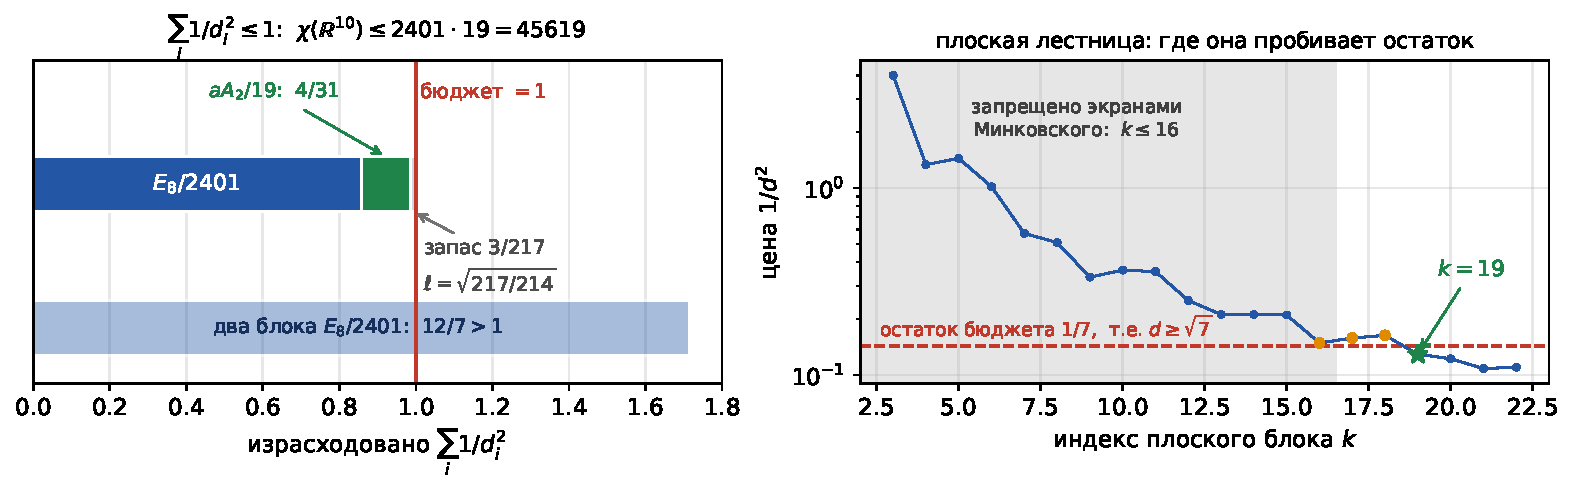
\includegraphics[width=\textwidth]{fig_budget.pdf}
\caption{Слева: бюджет $\sum_i 1/d_i^2\le1$ как полоса длины~1. Блок $E_8/2401$
занимает $6/7$, плоский проставок индекса~19 --- $4/31$, остаток $3/217$ и даёт
ширину $\ell=\sqrt{217/214}$. Два блока $E_8/2401$ в бюджет не помещаются
($12/7>1$) --- поэтому в произведении может быть лишь один эффективный блок.
Справа: плоская лестница цены $1/d^2$ по индексу; горизонталь --- остаток
бюджета $1/7$, серая зона запрещена экранами (\S\ref{ssec:planefloor}).}
\label{fig:budget}
\end{figure}

\subsection{Что закрыто}
\label{ssec:prodneg}

\textbf{$7^6$ в размерности 12 недостижимо.} Пока была доказана лишь нижняя
оценка $D\ge\sqrt{7/3}\lambda_1$, оставался шанс, что у решётки
Коксетера--Тодда настоящее $D$ больше (тогда $\chi(\R^{12})\le7^6=117649$ вместо
$3^{12}=531441$). Теорема~\ref{thm:eis} закрывает вопрос сразу:
$D\bigl((3+\omega)K_{12}\bigr)=\sqrt{7/3}\,\lambda_1$, то есть ровно нижняя граница через проекцию на
плоскость, при требуемом $\diam=2\sqrt{8/3}=3{,}265986$. Прямой счёт, которым это было
установлено первоначально, сохраняем как независимую проверку: перебор
$85\,680$ векторов $(3+\omega)K_{12}$ против полупространств \emph{всех} $756$
минимальных векторов даёт $D_{\min}=3{,}055050463=\sqrt{7/3}\cdot2$. Значит
эйзенштейнов путь в $\R^{12}$ требует именно $\rho\le\sqrt{7/3}=1{,}5275$, тогда
как $\rho(K_{12})=1{,}6330$. Более того, $(3+\omega)K_{12}$ с индексом
$7^6=117\,649$ лежит \emph{ниже} оболочечного пола $177\,979$.

\textbf{Эйзенштейнов путь в комплексном ранге~$5$.} Индекс $7^{n/2}$ требует
$\rho\le\sqrt{7/3}$. Наилучший тернарный код длины~$5$ с $d\ge3$ имеет $k=2$
(у кода $[5,3,3]_3$ проверочная матрица имела бы пять попарно
непропорциональных столбцов в $\mathbb F_3^2$, а таких лишь четыре), и
решётка даёт
по прямому измерению $D_{\min}=\sqrt7$ и $d=0{,}8367$, то есть
$\rho=\sqrt{7/3}/d\approx1{,}826$; поиск по всем эрмитовым формам ранга~5
(\path{audit-data/results/eisenstein_rank5_cma.json}) не опускает $\rho$
ниже $1{,}7496$. Вместе с $K_{12}$ это распространяет частичный
отрицательный ответ на открытый вопрос~2 работы~\cite{ABPR} с ранга~$6$ на
ранг~$5$.

\textbf{Слой ранга 2 не проходит (численно).} Естественное продолжение ---
надстроить над $E_8/2401$ слоевую решётку ранга~2, получив
$\chi(\R^{12})\le2401\,N(\alpha)^2$. Попутно найдена лучшая эйзенштейнова
решётка ранга~2: оптимизация по эрмитовым формам даёт $\rho=1{,}3626553$, что
лучше $D_4$ ($\sqrt2$) и $A_2\oplus A_2$ ($1{,}6330$). Тем не менее численный
фронтир встаёт на $0{,}79$--$0{,}94$, причём увеличение бюджета оптимизации
ухудшает результат: ландшафт рваный.

Причина установлена подсчётом и показана на рис.~\ref{fig:shells}: поправки
обязаны вытолкнуть за диаметр \emph{каждый} класс слоевой подрешётки, попавший
в окно $|c|\le\diam+\lambda_1$. В плоскости таких классов ровно шесть --- одна
орбита действия $\omega$, а следующая оболочка лежит далеко за окном; в ранге~2
их двадцать четыре, четыре орбиты, причём три почти вырождены по длине
($3{,}2909$, $3{,}2913$, $3{,}2916$) и должны быть вытолкнуты одновременно.
Отсюда видно напряжение, которое иначе нечем было бы заметить: малое $\rho$ означает
<<круглую>> решётку, а круглая решётка имеет много векторов почти равной длины,
то есть много связывающих орбит. Слою нужны одновременно малое~$\rho$ (бюджет)
и разреженные оболочки (выполнимость), и в ранге~1 второе даётся даром.

\begin{figure}[htbp]\centering
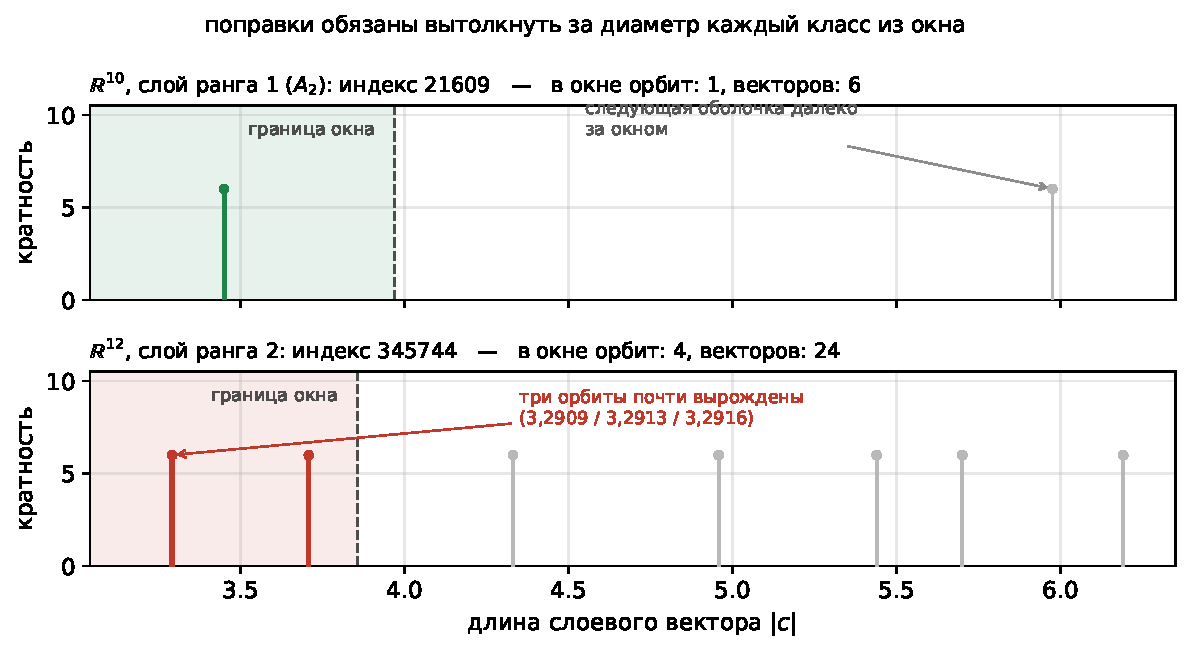
\includegraphics[width=\textwidth]{fig_shells.pdf}
\caption{Длины слоевых векторов подрешётки с кратностями. Сверху слой ранга~1
(размерность~10): в окне одна орбита, следующая оболочка далеко. Снизу слой
ранга~2 (размерность~12): четыре орбиты, три почти вырождены.}
\label{fig:shells}
\end{figure}

\textbf{$E_8$ --- локальный минимум $\rho$ (численно).} Поскольку узким местом
оказался разрыв восьмимерной лестницы между $2401$ ($d=1{,}0801$) и $6561$
($d=1{,}4142$), естественно спросить, нельзя ли поднять ширину самого блока,
взяв другую эйзенштейнову решётку. Отображение выигрыша прямое,
$d=\sqrt{7/3}/\rho$, и пороги в $\R^{10}$ таковы: $\rho\le1{,}4099$ даёт
проставок индекса~16 и произведение $38416$; $\rho\le1{,}3572$ --- индекс~13 и
$31213$; $\rho\le1{,}3229$ --- индекс~12 и $28812$; $\rho\le1{,}2472$ ---
индекс~9 и $21609$. У $E_8$ ровно $\rho=\sqrt2=1{,}4142$, до первого порога не
хватает $0{,}3\%$, а объёмный пол упаковки $(1/\delta_8)^{1/8}=1{,}1870$ ничего
из этого не запрещает. Тем не менее ответ отрицательный: $E_8$ восстанавливается
из своего $\Z[\omega]$-базиса ($\rho=1{,}414213562$ ровно), и локальная
оптимизация из неё даёт только худшие значения --- $1{,}4198$, $1{,}4237$,
$1{,}4243$, $1{,}4241$ при малом шаге и $1{,}4602$, $1{,}4408$, $1{,}4351$,
$1{,}4374$ при большом. Разрыв восьмимерной лестницы придётся брать
неэйзенштейновыми подрешётками, а не деформацией родительской решётки.
